%!TeX root=../pridetop.tex
\chapter[Chapter \thechapter]{}
	
	
\begin{figure}[t!]
\centering
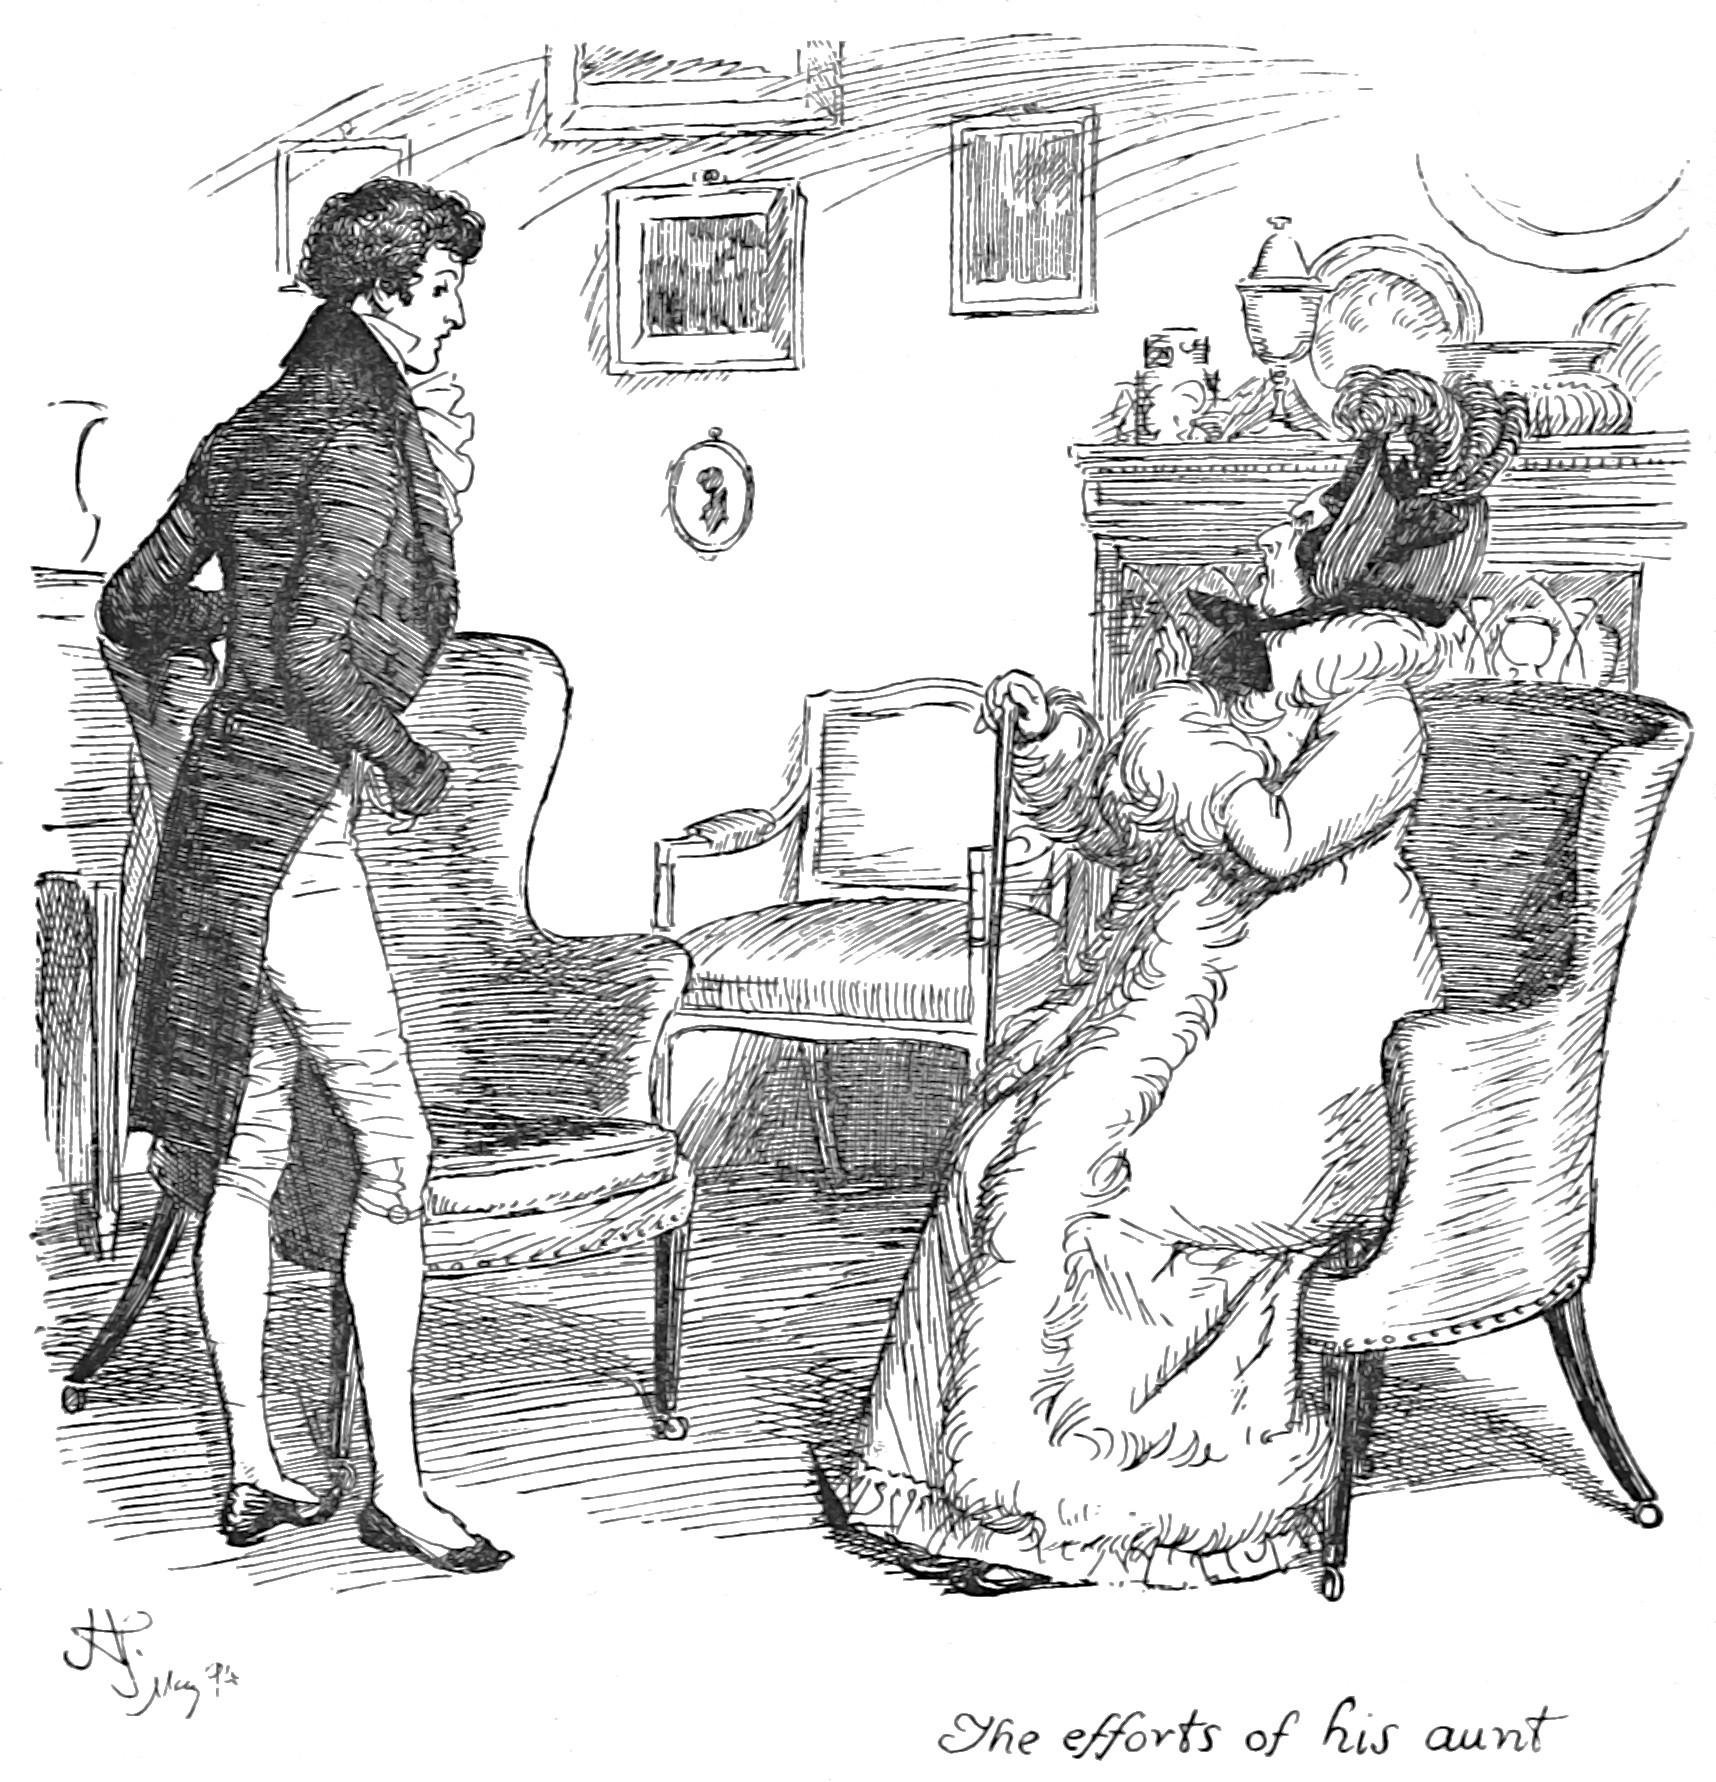
\includegraphics[width=.9\linewidth]{58top}
\captionlistentry{The efforts of his aunt}
\end{figure}


\lettrine[lines=6,image=true,findent=2pt]{initials/chap58instead}{of} receiving any such letter of excuse from his friend, as Elizabeth half expected Mr Bingley to do, he was able to bring Darcy with him to Longbourn before many days had passed after Lady Catherine's visit. The gentlemen arrived early; and, before Mrs Bennet had time to tell him of their having seen his aunt, of which her daughter sat in momentary dread, Bingley, who wanted to be alone with Jane, proposed their all walking out. It was agreed to. Mrs Bennet was not in the habit of walking, Mary could never spare time, but the remaining five set off together. Bingley and Jane, however, soon allowed the others to outstrip them. They lagged behind, while Elizabeth, Kitty, and Darcy were to entertain each other. Very little was said by either; Kitty was too much afraid of him to talk; Elizabeth was secretly forming a desperate resolution; and, perhaps, he might be doing the same.

They walked towards the Lucases', because Kitty wished to call upon Maria; and as Elizabeth saw no occasion for making it a general concern, when Kitty left them she went boldly on with him alone. Now was the moment for her resolution to be executed; and while her courage was high, she immediately said,—

»Mr Darcy, I am a very selfish creature, and for the sake of giving relief to my own feelings care not how much I may be wounding yours. I can no longer help thanking you for your unexampled kindness to my poor sister. Ever since I have known it I have been most anxious to acknowledge to you how gratefully I feel it. Were it known to the rest of my family I should not have merely my own gratitude to express.«

»I am sorry, exceedingly sorry,« replied Darcy, in a tone of surprise and emotion, »that you have ever been informed of what may, in a mistaken light, have given you uneasiness. I did not think Mrs Gardiner was so little to be trusted.«

»You must not blame my aunt. Lydia's thoughtlessness first betrayed to me that you had been concerned in the matter; and, of course, I could not rest till I knew the particulars. Let me thank you again and again, in the name of all my family, for that generous compassion which induced you to take so much trouble, and bear so many mortifications, for the sake of discovering them.«

»If you \textit{will} thank me,« he replied, »let it be for yourself alone. That the wish of giving happiness to you might add force to the other inducements which led me on, I shall not attempt to deny. But your \textit{family} owe me nothing. Much as I respect them, I believe I thought only of \textit{you}.«

Elizabeth was too much embarrassed to say a word. After a short pause, her companion added, »You are too generous to trifle with me. If your feelings are still what they were last April, tell me so at once. \textit{My} affections and wishes are unchanged; but one word from you will silence me on this subject for ever.«

Elizabeth, feeling all the more than common awkwardness and anxiety of his situation, now forced herself to speak; and immediately, though not very fluently, gave him to understand that her sentiments had undergone so material a change since the period to which he alluded, as to make her receive with gratitude and pleasure his present assurances. The happiness which this reply produced was such as he had probably never felt before; and he expressed himself on the occasion as sensibly and as warmly as a man violently in love can be supposed to do. Had Elizabeth been able to encounter his eyes, she might have seen how well the expression of heartfelt delight diffused over his face became him: but though she could not look she could listen; and he told her of feelings which, in proving of what importance she was to him, made his affection every moment more valuable.

They walked on without knowing in what direction. There was too much to be thought, and felt, and said, for attention to any other objects. She soon learnt that they were indebted for their present good understanding to the efforts of his aunt, who \textit{did} call on him in her return through London, and there relate her journey to Longbourn, its motive, and the substance of her conversation with Elizabeth; dwelling emphatically on every expression of the latter, which, in her Ladyship's apprehension, peculiarly denoted her perverseness and assurance, in the belief that such a relation must assist her endeavours to obtain that promise from her nephew which \textit{she} had refused to give. But, unluckily for her Ladyship, its effect had been exactly contrariwise.

»It taught me to hope,« said he, »as I had scarcely ever allowed myself to hope before. I knew enough of your disposition to be certain, that had you been absolutely, irrevocably decided against me, you would have acknowledged it to Lady Catherine frankly and openly.«

Elizabeth coloured and laughed as she replied, »Yes, you know enough of my \textit{frankness} to believe me capable of \textit{that}. After abusing you so abominably to your face, I could have no scruple in abusing you to all your relations.«

»What did you say of me that I did not deserve? For though your accusations were ill-founded, formed on mistaken premises, my behaviour to you at the time had merited the severest reproof. It was unpardonable. I cannot think of it without abhorrence.«

»We will not quarrel for the greater share of blame annexed to that evening,« said Elizabeth. »The conduct of neither, if strictly examined, will be irreproachable; but since then we have both, I hope, improved in civility.«

»I cannot be so easily reconciled to myself. The recollection of what I then said, of my conduct, my manners, my expressions during the whole of it, is now, and has been many months, inexpressibly painful to me. Your reproof, so well applied, I shall never forget: »Had you behaved in a more gentlemanlike manner.« Those were your words. You know not, you can scarcely conceive, how they have tortured me; though it was some time, I confess, before I was reasonable enough to allow their justice.«

»I was certainly very far from expecting them to make so strong an impression. I had not the smallest idea of their being ever felt in such a way.«

»I can easily believe it. You thought me then devoid of every proper feeling, I am sure you did. The turn of your countenance I shall never forget, as you said that I could not have addressed you in any possible way that would induce you to accept me.«

»Oh, do not repeat what I then said. These recollections will not do at all. I assure you that I have long been most heartily ashamed of it.«

Darcy mentioned his letter. »Did it,« said he,—»did it \textit{soon} make you think better of me? Did you, on reading it, give any credit to its contents?«

She explained what its effects on her had been, and how gradually all her former prejudices had been removed.

»I knew,« said he, »that what I wrote must give you pain, but it was necessary. I hope you have destroyed the letter. There was one part, especially the opening of it, which I should dread your having the power of reading again. I can remember some expressions which might justly make you hate me.«

»The letter shall certainly be burnt, if you believe it essential to the preservation of my regard; but, though we have both reason to think my opinions not entirely unalterable, they are not, I hope, quite so easily changed as that implies.«

»When I wrote that letter,« replied Darcy, »I believed myself perfectly calm and cool; but I am since convinced that it was written in a dreadful bitterness of spirit.«

»The letter, perhaps, began in bitterness, but it did not end so. The adieu is charity itself. But think no more of the letter. The feelings of the person who wrote and the person who received it are now so widely different from what they were then, that every unpleasant circumstance attending it ought to be forgotten. You must learn some of my philosophy. Think only of the past as its remembrance gives you pleasure.«

»I cannot give you credit for any philosophy of the kind. \textit{Your} retrospections must be so totally void of reproach, that the contentment arising from them is not of philosophy, but, what is much better, of ignorance. But with \textit{me}, it is not so. Painful recollections will intrude, which cannot, which ought not to be repelled. I have been a selfish being all my life, in practice, though not in principle. As a child I was taught what was \textit{right}, but I was not taught to correct my temper. I was given good principles, but left to follow them in pride and conceit. Unfortunately an only son (for many years an only \textit{child}), I was spoiled by my parents, who, though good themselves, (my father particularly, all that was benevolent and amiable,) allowed, encouraged, almost taught me to be selfish and overbearing, to care for none beyond my own family circle, to think meanly of all the rest of the world, to \textit{wish} at least to think meanly of their sense and worth compared with my own. Such I was, from eight to eight-and-twenty; and such I might still have been but for you, dearest, loveliest Elizabeth! What do I not owe you! You taught me a lesson, hard indeed at first, but most advantageous. By you, I was properly humbled. I came to you without a doubt of my reception. You showed me how insufficient were all my pretensions to please a woman worthy of being pleased.«

»Had you then persuaded yourself that I should?«

»Indeed I had. What will you think of my vanity? I believed you to be wishing, expecting my addresses.«

»My manners must have been in fault, but not intentionally, I assure you. I never meant to deceive you, but my spirits might often lead me wrong. How you must have hated me after \textit{that} evening!«

»Hate you! I was angry, perhaps, at first, but my anger soon began to take a proper direction.«

»I am almost afraid of asking what you thought of me when we met at Pemberley. You blamed me for coming?«

»No, indeed, I felt nothing but surprise.«

»Your surprise could not be greater than \textit{mine} in being noticed by you. My conscience told me that I deserved no extraordinary politeness, and I confess that I did not expect to receive \textit{more} than my due.«

»My object \textit{then},« replied Darcy, »was to show you, by every civility in my power, that I was not so mean as to resent the past; and I hoped to obtain your forgiveness, to lessen your ill opinion, by letting you see that your reproofs had been attended to. How soon any other wishes introduced themselves, I can hardly tell, but I believe in about half an hour after I had seen you.«

He then told her of Georgiana's delight in her acquaintance, and of her disappointment at its sudden interruption; which naturally leading to the cause of that interruption, she soon learnt that his resolution of following her from Derbyshire in quest of her sister had been formed before he quitted the inn, and that his gravity and thoughtfulness there had arisen from no other struggles than what such a purpose must comprehend.

She expressed her gratitude again, but it was too painful a subject to each to be dwelt on farther.

After walking several miles in a leisurely manner, and too busy to know anything about it, they found at last, on examining their watches, that it was time to be at home.

»What could have become of Mr Bingley and Jane?« was a wonder which introduced the discussion of \textit{their} affairs. Darcy was delighted with their engagement; his friend had given him the earliest information of it.

»I must ask whether you were surprised?« said Elizabeth.

»Not at all. When I went away, I felt that it would soon happen.«

»That is to say, you had given your permission. I guessed as much.« And though he exclaimed at the term, she found that it had been pretty much the case.

»On the evening before my going to London,« said he, »I made a confession to him, which I believe I ought to have made long ago. I told him of all that had occurred to make my former interference in his affairs absurd and impertinent. His surprise was great. He had never had the slightest suspicion. I told him, moreover, that I believed myself mistaken in supposing, as I had done, that your sister was indifferent to him; and as I could easily perceive that his attachment to her was unabated, I felt no doubt of their happiness together.«

Elizabeth could not help smiling at his easy manner of directing his friend.

»Did you speak from your own observation,« said she, »when you told him that my sister loved him, or merely from my information last spring?«

»From the former. I had narrowly observed her, during the two visits which I had lately made her here; and I was convinced of her affection.«

»And your assurance of it, I suppose, carried immediate conviction to him.«

»It did. Bingley is most unaffectedly modest. His diffidence had prevented his depending on his own judgment in so anxious a case, but his reliance on mine made everything easy. I was obliged to confess one thing, which for a time, and not unjustly, offended him. I could not allow myself to conceal that your sister had been in town three months last winter, that I had known it, and purposely kept it from him. He was angry. But his anger, I am persuaded, lasted no longer than he remained in any doubt of your sister's sentiments. He has heartily forgiven me now.«

Elizabeth longed to observe that Mr Bingley had been a most delightful friend; so easily guided that his worth was invaluable; but she checked herself. She remembered that he had yet to learn to be laughed at, and it was rather too early to begin. In anticipating the happiness of Bingley, which of course was to be inferior only to his own, he continued the conversation till they reached the house. In the hall they parted.